\section{Further Experiments}\label{sec:apdx:additional_experiments}
In this section we provide additional experiments that are not included in the main manuscript due to space constraints.

\begin{figure}[H]
    \centering
    \subfigure[Balanced teacher and general (unbalanced) student]{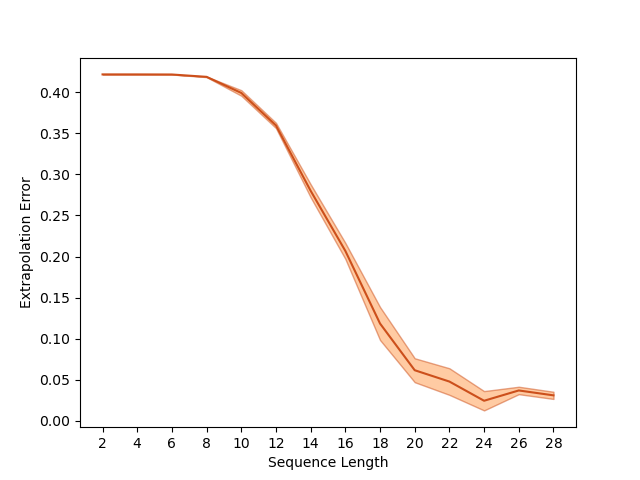
\includegraphics[width=0.49\textwidth]{figures/extrapolation_as_func_of_k_non_balanced_init.png}}
    \subfigure[Random (unbalanced) teacher and general (unbalanced) student]{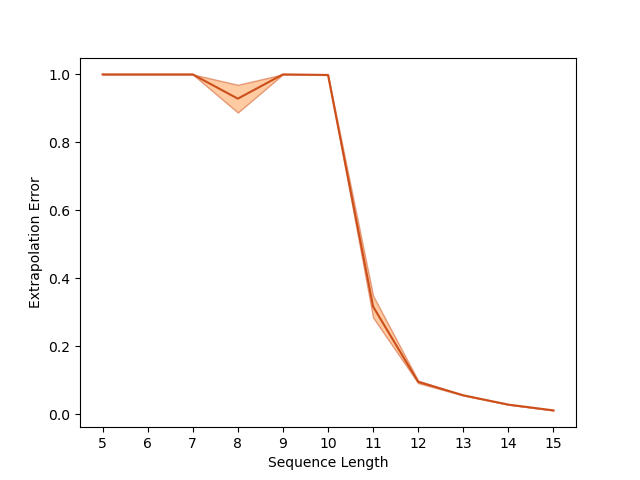
\includegraphics[width=0.49\textwidth]{figures/extrapolation_as_func_of_k_non_sym_teacher_init_1e-06.png}} 
    \caption{
    Extrapolation error as a function of the training sequence length $k$. (a) a balanced teacher with state dimensions $\hat{d}=5$ and a general (unbalanced and non-diagonal) student with $d=40$. (b) a random unbalanced teacher (see \Secref{sec:apdx:unbalanced_teacher}) with dimension $\hat{d}=5$, and a student that has a non-diagonal transition matrix and is trained with standard (small) initialization, with state dimension $d=50$. In both plots results are averaged over 3 seeds.}
    \label{fig:apdx_additional_experiments}
\end{figure}

\subsection{Balanced Teacher}\label{sec:apdx:balanced_teacher}
In \Secref{sec:exp:sym_teacher}, we have experimented with our proposed theoretical setup. In this section we provide additional figures and experiments.

\subsubsection{Unbalanced Student}\label{sec:apdx:unbalanced_student}

In this experiment we use the same balanced teacher with $\hat{d}=5$ as done in \Secref{sec:exp:sym_teacher}. Instead of the diagonal student with balanced initialization, we use a general (non-diagonal) student with weights sampled from a Gaussian with scale $10^{-5}$ and $d=40$. Results are depicted in \figref{fig:apdx_additional_experiments}(a). A similar phase transition phenomenon to the one in \figref{fig:phase_transition_v2} is found also here.


\subsubsection{Effect of the Initialization Scale}\label{sec:largeinit}

Proposition~\ref{prop:implicit_bias_for_balanced_init} provides theoretical support for the fact that under near-zero initialization, the learned RNN tends to balancedness, which according to theorems \ref{thm:exact_extrapolation} and~\ref{thm:main_result} guarantees extrapolation.
Below we empirically explore the impact of varying the initialization scale. We use the same setting as in \Secref{sec:apdx:unbalanced_student}, and repeat the experiment with different initialization scales for the students' weights.


\begin{figure}
\centering
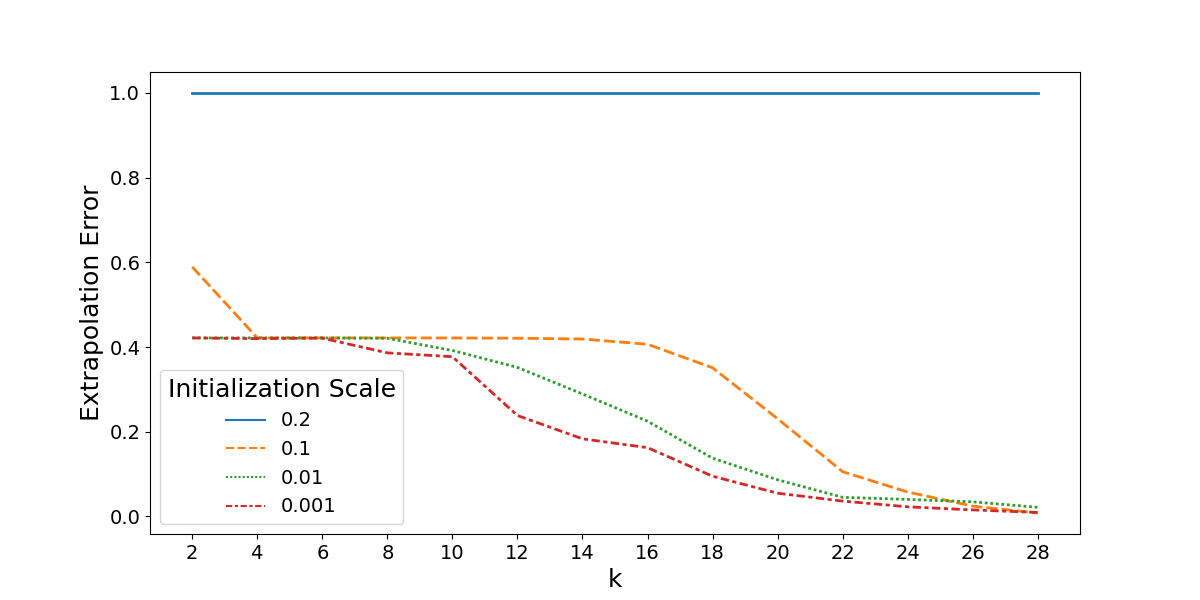
\includegraphics[width=0.75\textwidth]{figures/init_breaks2.png}
\caption{
Extrapolation error as a function of training sequence length $k$ for different initialization scales. Extrapolation error increases along with the scale of initialization.
}
\label{fig:init_breaks}
\end{figure}

As can be seen in \Figref{fig:init_breaks}, the extrapolation deteriorates for larger initialization scale, in the sense that it requires longer training sequences for getting good extrapolation error.  This suggests that the condition of small initialization required by our theory is not an artifact of our proof technique, but rather a necessary condition for extrapolation to occur.

\subsection{Unbalanced Teacher}\label{sec:apdx:unbalanced_teacher}
In \Secref{sec:exp:step_func}, we have tested the extrapolation with respect to a specific unbalanced teacher and have observed a similar phase transition as predicted by the theory of \Secref{sec:analysis} and empirical evaluation of \Secref{sec:exp:sym_teacher}. Here we show that the phase transition is not limited to the specific teacher discussed by testing with respect to a randomly generated unbalanced (non-diagonal) teacher (see \Secref{sec:apdx:unbalanced_teacher_generation}). The teacher is set to $\hat{d}=5$ and student to $d=50$. Results are presented in \figref{fig:apdx_additional_experiments}~(b). Here too we can observe the phase transition phenomena.


\subsection{Impulse Response Figures}
In \Secref{sec:experiments} we have presented the extrapolation performance in different settings. In order to better convey the meaning of extrapolating vs non-extrapolating solutions we present here figures of the impulse response of different models.

We start with the impulse response corresponding to the experiment described in \Secref{sec:exp:sym_teacher}. The figure depicts the balanced teacher with $\hat{d}=5$ and two selected students (with $d=40$), one trained with $k=10$ and the other with $k=20$.

\begin{figure}[H]
    \centering
    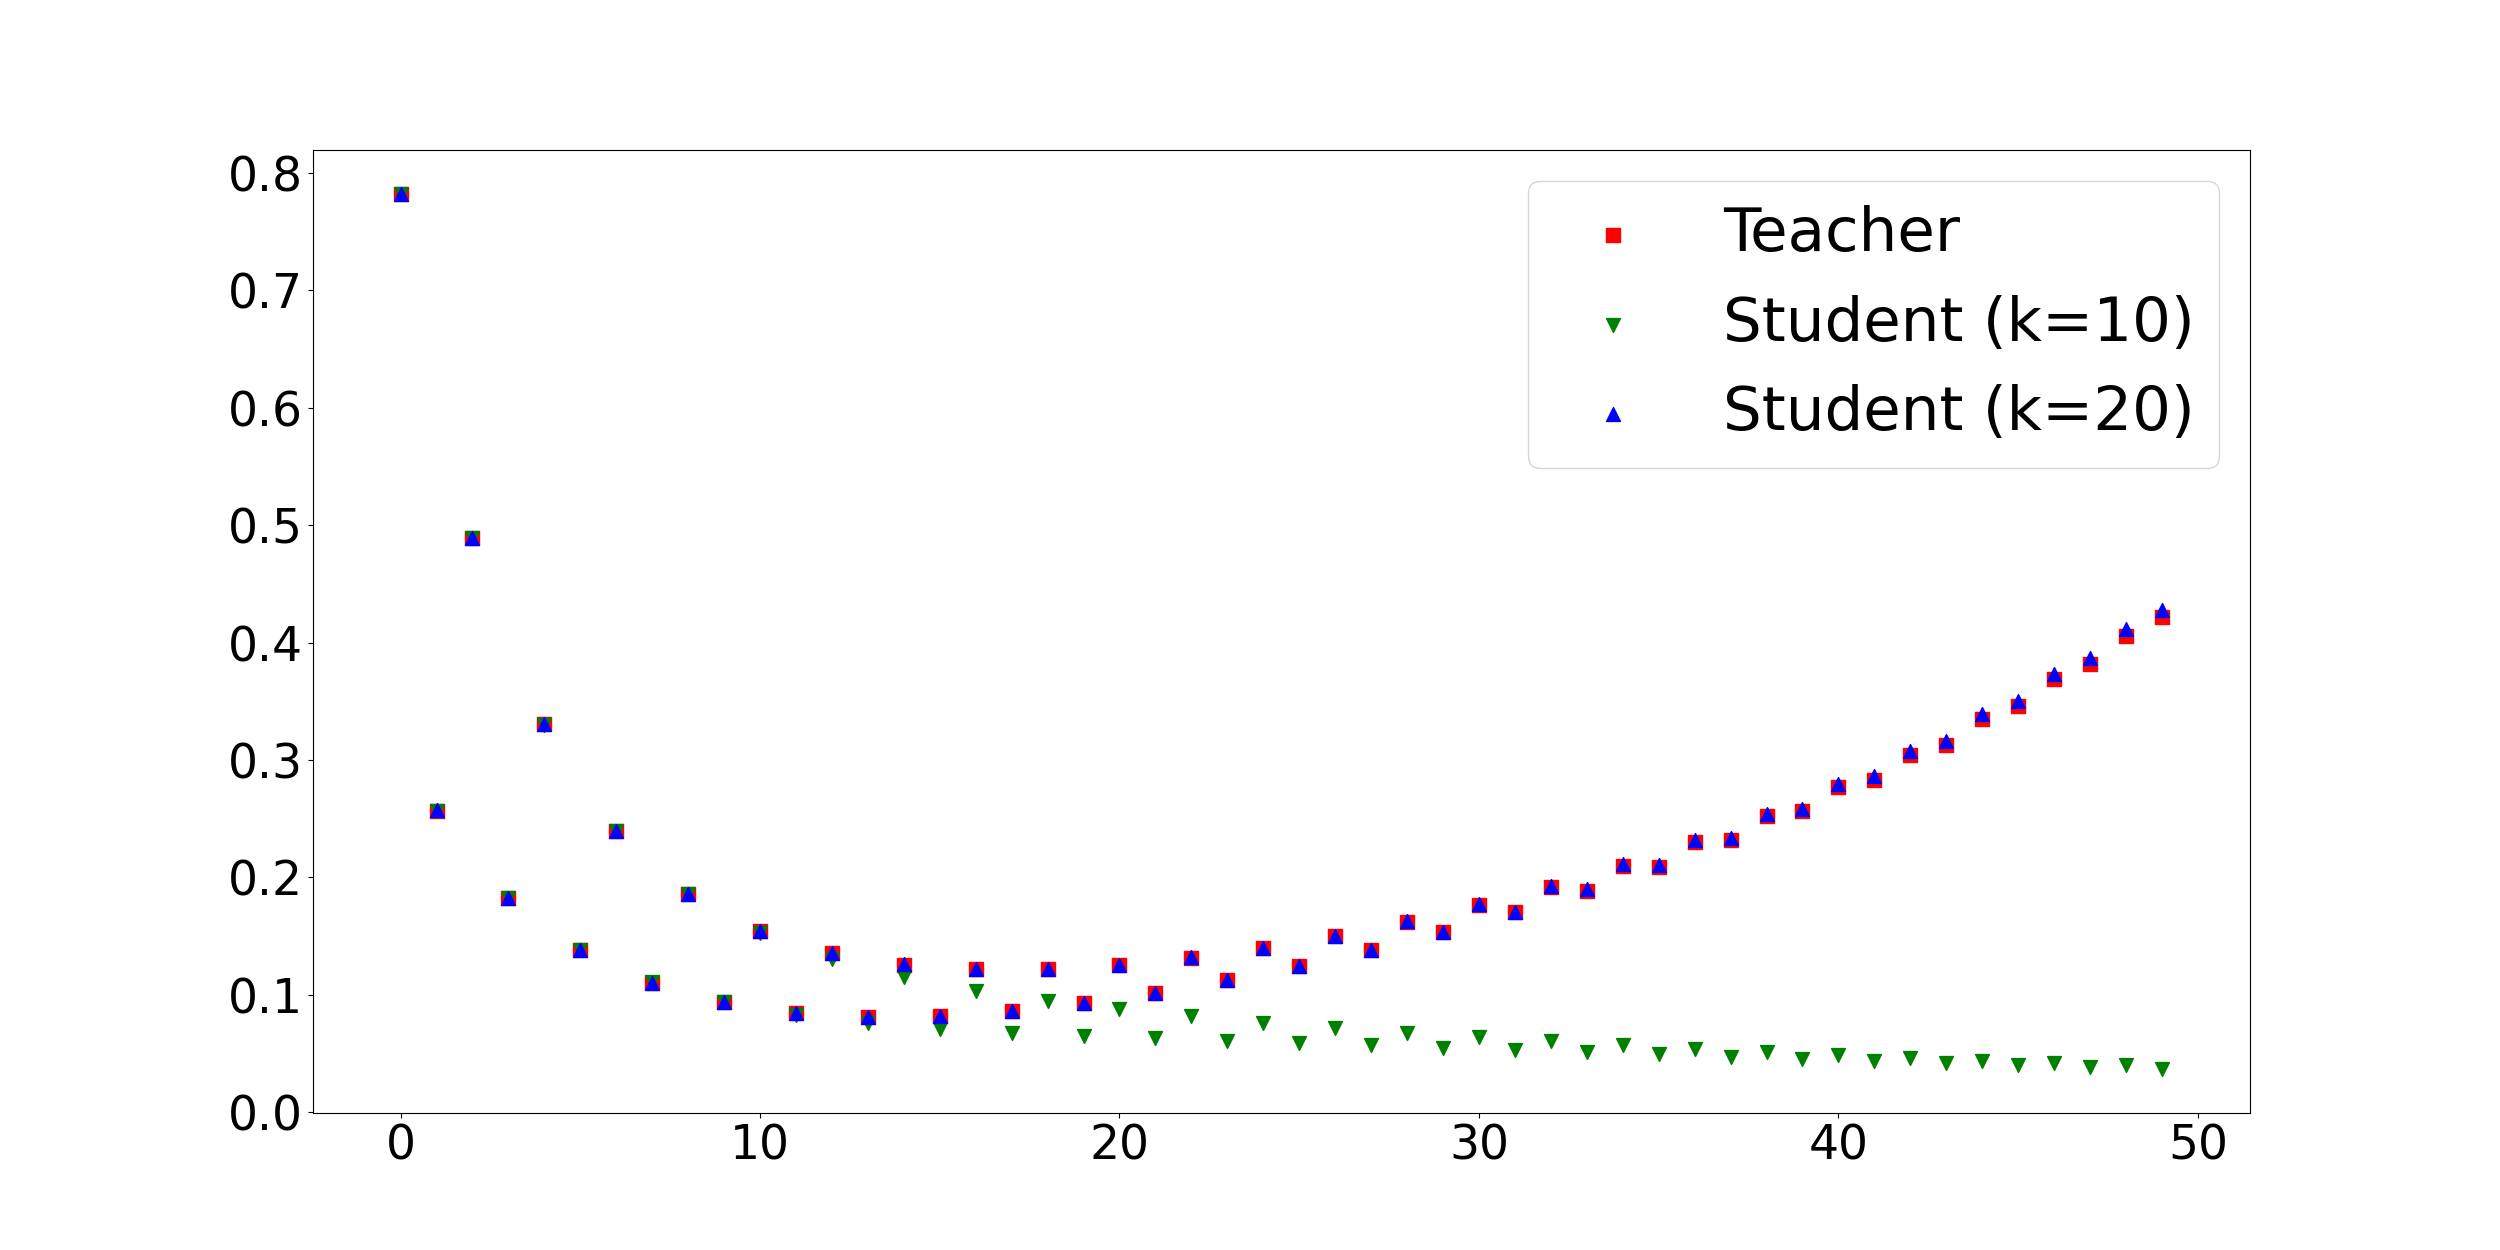
\includegraphics[width=0.8\textwidth]{figures/balanced_impulse_responses.png}
    \caption{\textbf{Balanced teacher and student impulse response}. Students trained with: $k=10,20$ with respect to the balanced teacher described in \Secref{sec:apdx:balanced_teacher_generation}. As can be seen, both students track the teacher up to the $k$ used in training, for $k=10$ there is no extrapolation for larger values of $k$, whereas $k=20$ tracks the teacher well beyond the sequence length used in training.}
    \label{fig:apdx:balanced_ir}
\end{figure}

We can see that the student trained with $k=10$ tracks the teacher several steps beyond the $10th$ time step and then decays to zero. For $k=20$ we can see near perfect extrapolation for the horizon evaluated.

Next we turn to \Secref{sec:exp:step_func} and depict the average impulse responses of the ``delay teacher'' and the students trained with respect to the mentioned teacher.

\begin{figure}[H]
    \centering
    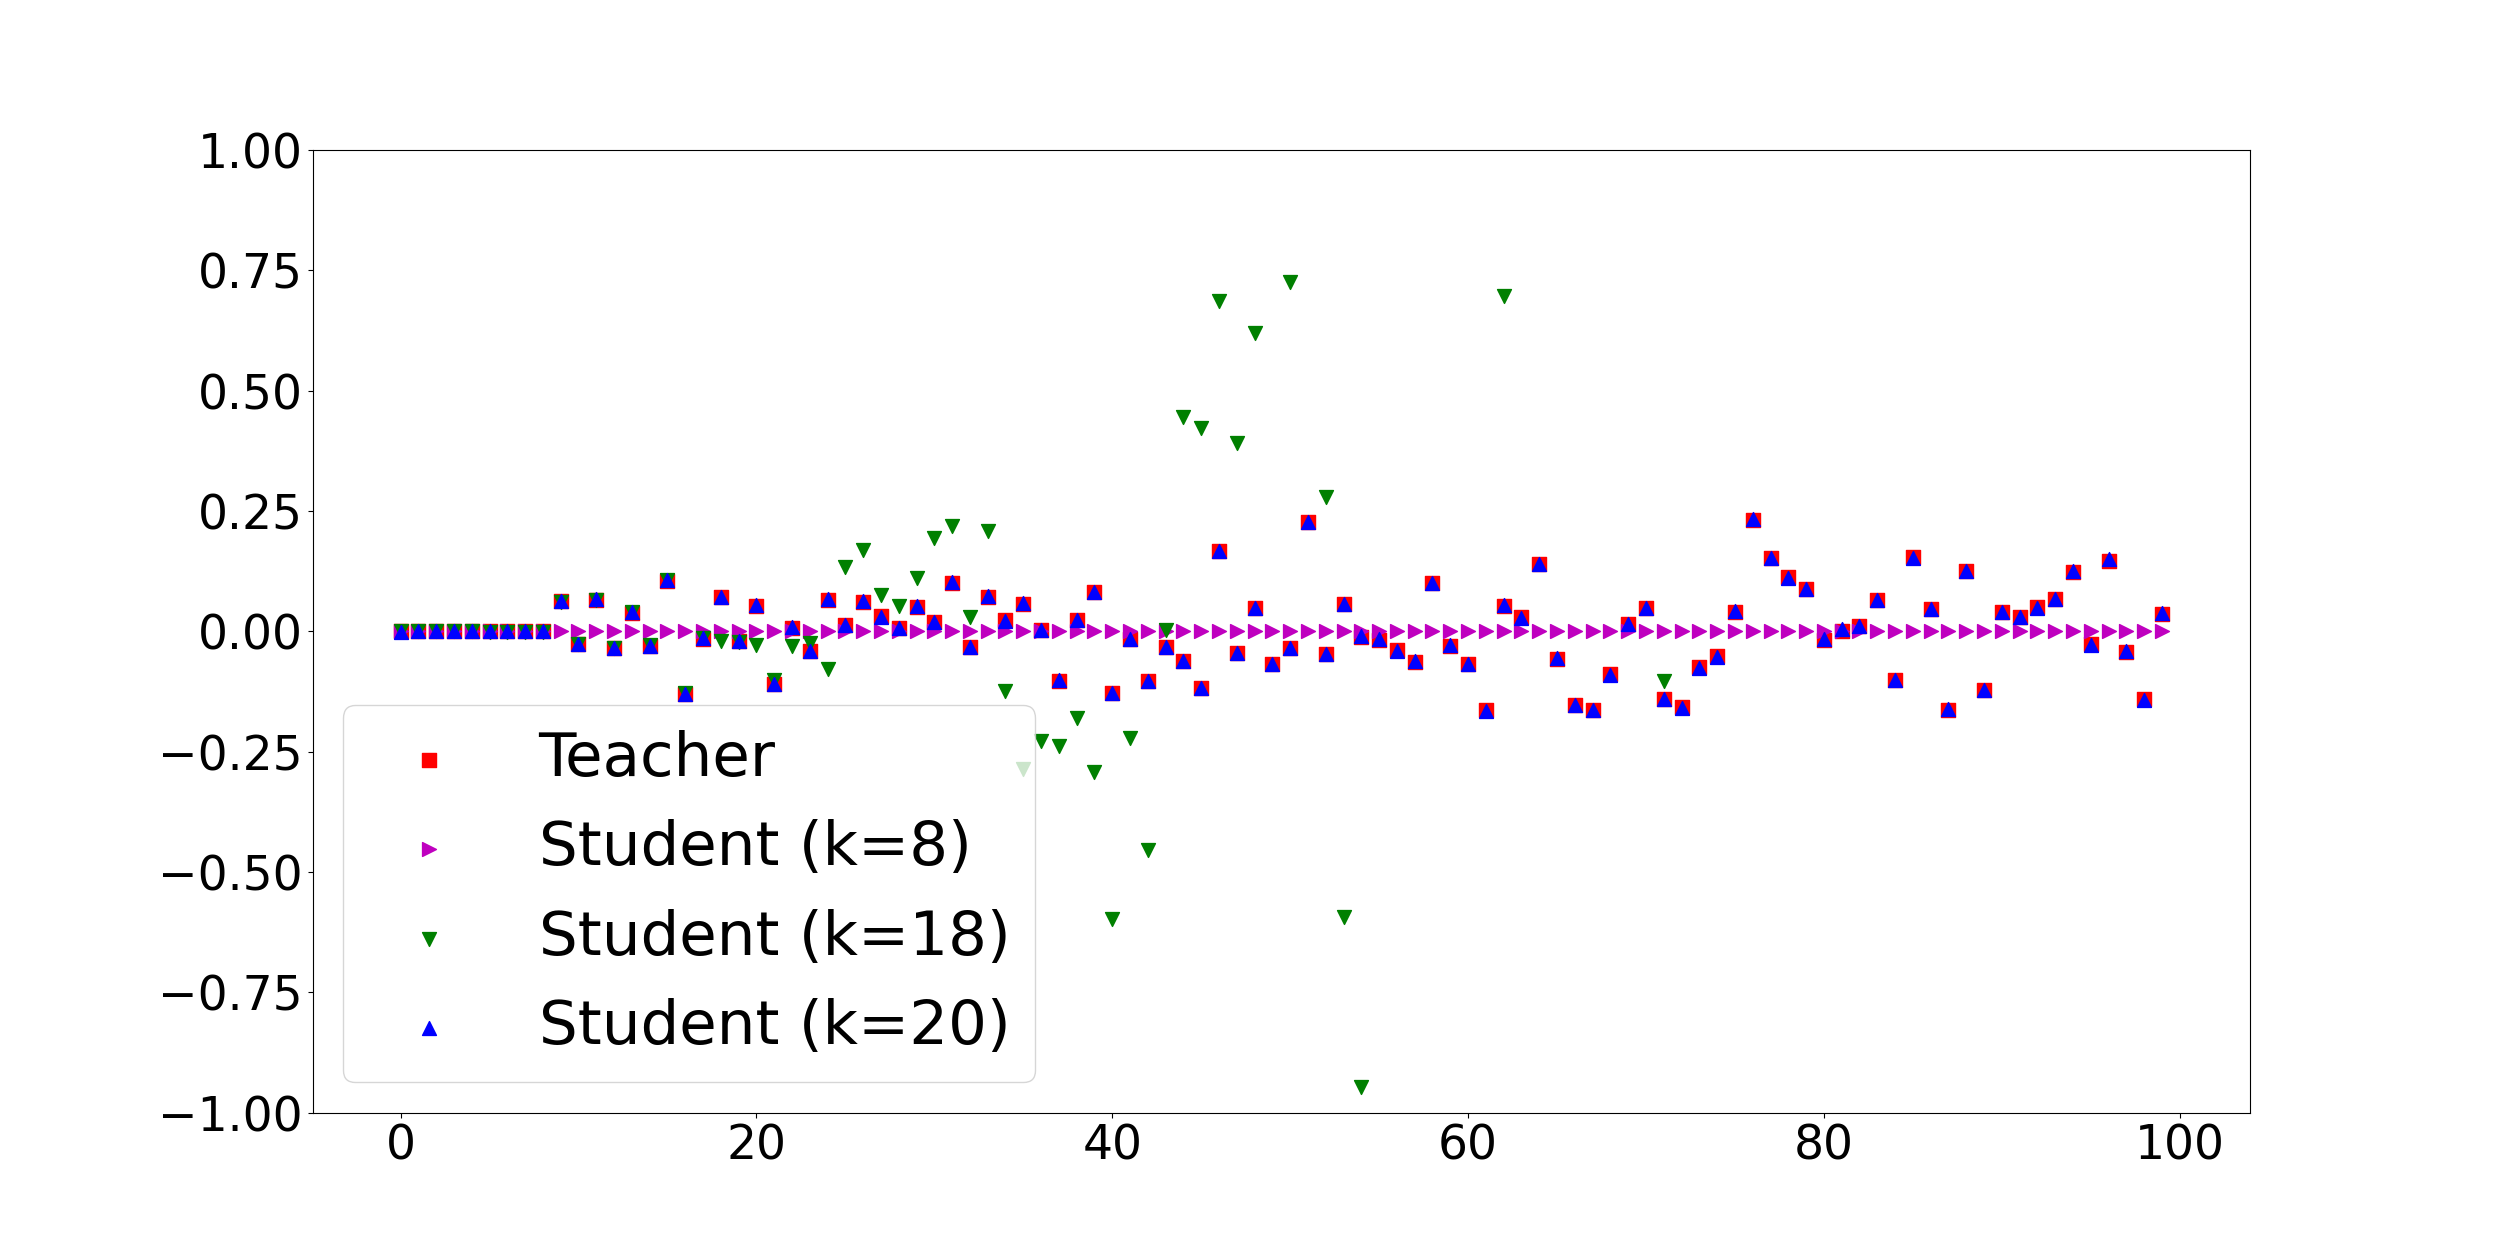
\includegraphics[width=0.8\textwidth]{figures/non_sym_impulse_responses.png}
    \caption{\textbf{Unbalanced teacher (delay) and student impulse response}. Students trained with: $k=8,18,20$ with respect to the unbalanced delay teacher described in \Secref{sec:apdx:unbalanced_teacher_generation}. We can see that for $k=18$ the student diverges for longer sequences while $k=20$ which is trained for merely two additional time steps extrapolates and tracks the teacher almost perfectly.}
    \label{fig:apdx:delay_teacher_ir}
\end{figure}

Since the teacher here has $\hat{d}=10$, a model trained with $k=8$ is trained with respect to the zero impulse response (see \Secref{sec:apdx:unbalanced_teacher_generation} for details on delay teacher), and as expected results with the `zero' solution. we can see that for $k=18$ the student diverges from the teacher shortly after the $18th$ time step. For $k=20$ we can see near perfect extrapolation up to the horizon considered.

\section{Implementation Details}\label{sec:apdx:impl_details}

All the experiments are implemented using PyTorch.

\subsection{Optimization}
In \Secref{sec:exp:sym_teacher} we optimize the population loss, which entails minimizing \Eqref{eq:population_loss} with respect to the parameters of the learned model. We use 15K optimization steps with Adam optimizer and a learning rate of $10^{-3}$. In this experiment, the results were not sensitive to the initialization scale of the (balanced) student.
In \Secref{sec:exp:step_func} and \Secref{sec:exp:non_linear_teacher} in the experiments that involve minimizing the empirical loss, we use 50K optimization steps with early stopping (most experiments required less than 10K steps). The batch size is set to $100$, data is sampled from a Gaussian with zero mean and scale of $1$. Experiments were not sensitive to most hyper-parameters other than learning rate and initialization scale. The examination of the effect of initialization scale presented in \Secref{sec:largeinit} is done with learning rate scheduler \verb|torch.optim.lr_scheduler.MultiStepLR| using milestones at $[5000,10000,15000,30000]$ and a decaying factor of $\gamma=0.1$.


\subsection{Teacher Generation}\label{sec:apdx:teacher_gen}
One of the main challenges in empirically evaluating extrapolation is that randomly sampling weights from a Gaussian distribution may result with an RNN of lower effective rank (i.e. the resulting RNN may be accurately approximated with another RNN with a smaller hidden dimension). We will now describe the teacher generation scheme for the different experiments.

\subsubsection{Balanced Teacher Generation}\label{sec:apdx:balanced_teacher_generation}
A balanced teacher consists of $d$ entries corresponding to the diagonal teacher and $d$ entries representing $\hat{\mB}=\hat{\mC}^\top$. In order to avoid cases of rapid decay in the impulse response on the one hand, and exponential growth on the other, we set the eigenvalues to distribute uniformly between $0.6$ and $1.05$. The values of $\hat{\mB}$ and $\hat{\mC}$ are randomly sampled from a Gaussian around 0.5 and scale 1 and then normalized such that $\hat{\mC}\hat{\mB}=1$.

\subsubsection{Unbalanced Teacher Generation}\label{sec:apdx:unbalanced_teacher_generation}
In this experiment, the teacher has a general (non-symmetrid) matrix $\hat{\mA}$ and $\hat{\mB}\neq\hat{\mC}^\top$. We  set the weights as described next.

\paragraph{Delay Teacher}
A `delay' teacher has an impulse response of $1$ at time step $i=\hat{d}-1$, that is, the teacher has an impulse response of $(0,\dots,0,1,0,\dots)$. In order to generate the mentioned impulse response we set the weights as follows,

\begin{equation}\label{eq:step_func}
    \mA=\begin{pmatrix}
    0 & 1 &   & 0 \\
      &   & \ddots &   \\
    0 & 0 &   & 1 \\
    0 & 0 &   & 0
    \end{pmatrix},\; \mB=\begin{pmatrix}
    0 \\
    \vdots\\
    0\\
    1
    \end{pmatrix}, \text{ and } \mC^\top=\begin{pmatrix}
    1 \\
    0 \\
    \vdots\\
    0
    \end{pmatrix}.
\end{equation}

Note that $\mB,\mC$ above are set to extract the last entry of the first row of $\mA^i$ and $\mA$ is a Nilpotent shift matrix. It is straightforward to verify that $\mC\mA^i\mB=1$ for $i=\hat{d}-1$ and $0$ otherwise.

\paragraph{Random Unbalanced Teacher}
The second unbalanced teacher is randomly generated. In order to avoid the caveats mentioned in \Secref{sec:apdx:balanced_teacher}, we randomly sample the diagonal (from a Gaussian with zero mean and scale $0.1$) and super diagonal (from a Gaussian with mean $0.7$ and scale $0.1$) of $A$. We set $B,C$ as in \eqref{eq:step_func}. The structure of $\mA$ ensures similar properties to that of the delayed teacher, specifically, that the first entries of the impulse response is zero and the teacher is `revealed' only after $\hat{d}$ time steps.

\subsubsection{Non-Linear Teacher Generation}\label{sec:apdx:gru_teacher_generation}
As opposed to the linear teacher discussed in previous sections, when the teacher is a Gated Recurrent Units (GRU), it is unclear how to generate a non-trivial teacher. When randomly generating a teacher GRU the result is either a trivial model that quickly decays to zero or a teacher with an exploding impulse response (depending on the scale of the initialization). In order to produce a teacher with interesting extrapolation behaviour, we initialize a model with an initialization scale of $10^{-6}$ and train for $1000$ step the model to mimic an arbitrarily chosen impulse response. The result of the mentioned procedure is a teacher GRU with non-trivial behaviour.  \figref{fig:gru_extrapolation}(b) shows that we get with this non-trivial teacher the phase transition phenomena as described in \Secref{sec:exp:non_linear_teacher}.

\subsection{Extrapolation Error}\label{sec:apdx:extrapolation_error}
The concept of extrapolation is very intuitive, and yet it does not admit any standard error measure. A proper extrapolation error measure should: (a) capture fine differences between two models with good extrapolation behaviour; and on the other hand, (b) be insensitive to the scale in which two non-extrapolating model explode. 
A natural approach which we take here is to report the $\ell_{\infty}$ norm difference on the tail of the impulse response. A model is considered non-extrapolating if the extrapolation error is worse than the extrapolation error of a trivial solution which has an impulse response of zeros.